\documentclass[a4paper,10pt,titlepage]{article}
\usepackage[pdftex]{graphicx}
\setlength{\parindent}{0in}
\begin{document}
\section{Glossery}
	\textbf{Event}
	Something predicted to happen at some point.
	
\section{Vision}
	The purpose of this product is to make browsing, management and sharing easy for people with little or no knowledge about interaction with networks or computers. Performance shall be reasonable and use of the application shall not expose any security threats, unless prevention compromises usability or reliability.
	
\section{User cases}
	\textbf{Name}
	View calender
	\\
	\textbf{Scope}
	Calender client
	\\
	\textbf{Level}
	User goal
	\\
	\textbf{Primary Actor}
	User
	\\
	\textbf{Stakeholders and Interests}
	User
	\\
	\textbf{Precondition}
	User is connected to database.
	 User has logged on.
	\\
	\textbf{Postcondition}
	\\
	\textbf{Main Success Scenario}
	User gets the desired information.
	\\
	\textbf{Extensions}
	No database connection returns error
	\\
	\textbf{Special Requirements}
	\\
	
	\textbf{Name}
	Create event
	\\
	\textbf{Scope}
	Calender client
	\\
	\textbf{Level}
	User goal
	\\
	\textbf{Primary Actor}
	User
	\\
	\textbf{Stakeholders and Interests}
	User
	\\
	\textbf{Precondition}
	User is connected to database.
	User has logged on.
	\\
	\textbf{Postcondition}
	An event has been created in the database and the view is updated
	\\
	\textbf{Main Success Scenario}
	User creates the desired event
	\\
	\textbf{Extensions}
	No database connection returns error
	\\
	\textbf{Special Requirements}
	\\
	
	\textbf{Name}
	Delete event
	\\
	\textbf{Scope}
	Calender client
	\\
	\textbf{Level}
	User goal
	\\
	\textbf{Primary Actor}
	User
	\\
	\textbf{Stakeholders and Interests}
	User
	\\
	\textbf{Precondition}
	User is connected to database.
	User has logged on.
	User has chosen a single event in the users personal calender.
	\\
	\textbf{Postcondition}
	the chosen event has been deleted in the database and the view is updated.
	\\
	\textbf{Main Success Scenario}
	User deletes the desired event
	\\
	\textbf{Extensions}
	No database connection returns error
	\\
	\textbf{Special Requirements}
	\\
	
	\textbf{Name}
	Edit event
	\\
	\textbf{Scope}
	Calender client
	\\
	\textbf{Level}
	User goal
	\\
	\textbf{Primary Actor}
	User
	\\
	\textbf{Stakeholders and Interests}
	User
	\\
	\textbf{Precondition}
	User is connected to database.
	User has logged on.
	User has chosen a single event in the users personal calender.
	\\
	\textbf{Postcondition}
	The chosen event has been updated in the database and the view is updated
	\\
	\textbf{Main Success Scenario}
	User updates the desired event
	\\
	\textbf{Extensions}
	No database connection returns error
	\\
	\textbf{Special Requirements}
	\\
	
	\textbf{Name}
	User login
	\\
	\textbf{Scope}
	Calender client
	\\
	\textbf{Level}
	User goal
	\\
	\textbf{Primary Actor}
	User
	\\
	\textbf{Stakeholders and Interests}
	User
	\\
	\textbf{Precondition}
	User is connected to database.
	\\
	\textbf{Postcondition}
	The user has successfully logged on to the system
	\\
	\textbf{Main Success Scenario}
	User logs on to the system
	\\
	\textbf{Extensions}
	No database connection returns error
	Wrong e-mail address and/or paswords returns error and offers an opportunity to get the password sent by mail
	\\
	\textbf{Special Requirements}
	\\
	
	\textbf{Name}
	Share calender
	\\
	\textbf{Scope}
	Calender client
	\\
	\textbf{Level}
	User goal
	\\
	\textbf{Primary Actor}
	User
	\\
	\textbf{Stakeholders and Interests}
	User
	\\
	\textbf{Precondition}
	User is connected to database.
	User is logged on
	\\
	\textbf{Postcondition}
	The user has sent a share-invite to another user of the system
	\\
	\textbf{Main Success Scenario}
	The user successfully sends a share-invite to another user
	\\
	\textbf{Extensions}
	No database connection returns error
	The entered e-mail which the user wants to share the calender does not exist in the system. The user is presented with an error
	\\
	\textbf{Special Requirements}
	\\
	
	\textbf{Name}
	Accept request
	\\
	\textbf{Scope}
	Calender client
	\\
	\textbf{Level}
	User goal
	\\
	\textbf{Primary Actor}
	User
	\\
	\textbf{Stakeholders and Interests}
	User
	\\
	\textbf{Precondition}
	User is connected to database.
	User is logged on
	User has received an invite to see another users calender
	\\
	\textbf{Postcondition}
	The user has accepted the invite and is now able to see the shared calender. The view is updated.
	\\
	\textbf{Main Success Scenario}
	The user has access to see the shared calender
	\\
	\textbf{Extensions}
	No database connection returns error
	The user declines the invite, nothing happens
	\\
	\textbf{Special Requirements}
	
\section{Supplementary specification}
	The supplementary specification is structured using the FURPS+ model.
	\\ \\
	\textbf{Functionality:}
	The program shall support a minimum of functions.
	\begin{itemize}
	\item The functions shall support sharing of calenders, creation and modification of events and viewing.
	\item The functions shall be intuitively grouped.
	\\
	\end{itemize}
	\textbf{Usability:}
	The user shall be able to use the program with as little knowledge as possible, which raises the following requirements:
	\begin{itemize}
	\item The user should consider a minimum of options performing the desired task. This may compromise both performance and functionality.
	\item Anyone beyond the age of 12 shall be able to understand the program terminology. 
	\\
	\end{itemize}
	\textbf{Reliability:}
	The program shall be very reliable, even if it compromises security. Any error should result in recovery or crash, neither involving the user. Any crash or recovery must maintain the content of the database.
	\begin{itemize}
	\item The program shall be able to complete as many tasks as possible without internet connection.
	\\
	\end{itemize}
	\textbf{Performance:}
	The program shall have reasonable performance. This means that no operation shall take more than 2 seconds on a bandwidth with more than 2 mBit/s and a processor of more than 1 GHz.
	\\ \\
	\textbf{Supportability:}
	Functions shall be supported with a help page. The content should be limited because the intuitiveness and limited functionality makes it needless.
	\\ \\
\section{Operation Contracts}
	\textbf{Operation:}	newEvent(time:Date, description:String)
	\\ \\
	\textbf{References:}	User Cases:	Create new event
	\\ \\
	\textbf{Pre Conditions:}		
						User must be connected to the server
						User must be logged on to the system
					\\ \\
	\textbf{Post Conditions:}	
						An Event instance event was created (instance creation)
						event.ID is uniqe (Primary key established)
						event is associated with a Calendar, based on the users ID (association formed)
						event.description becomes description (attribute modefication)	
					\\ \\	
	\textbf{Operation:}	updateEvent(event:Event, command:String)
	\\ \\
	\textbf{References:}	User Cases:	Edit event, Delete event
	\\ \\
	\textbf{Pre Conditions:}
						User must be connected to the server
						User must be logged on to the system
						An exitsing Event must be selected
	\\ \\	
	\textbf{Post Conditions:}
						The incomming command has been executed on the target Event (instance modification)
						
						
\section{Models}
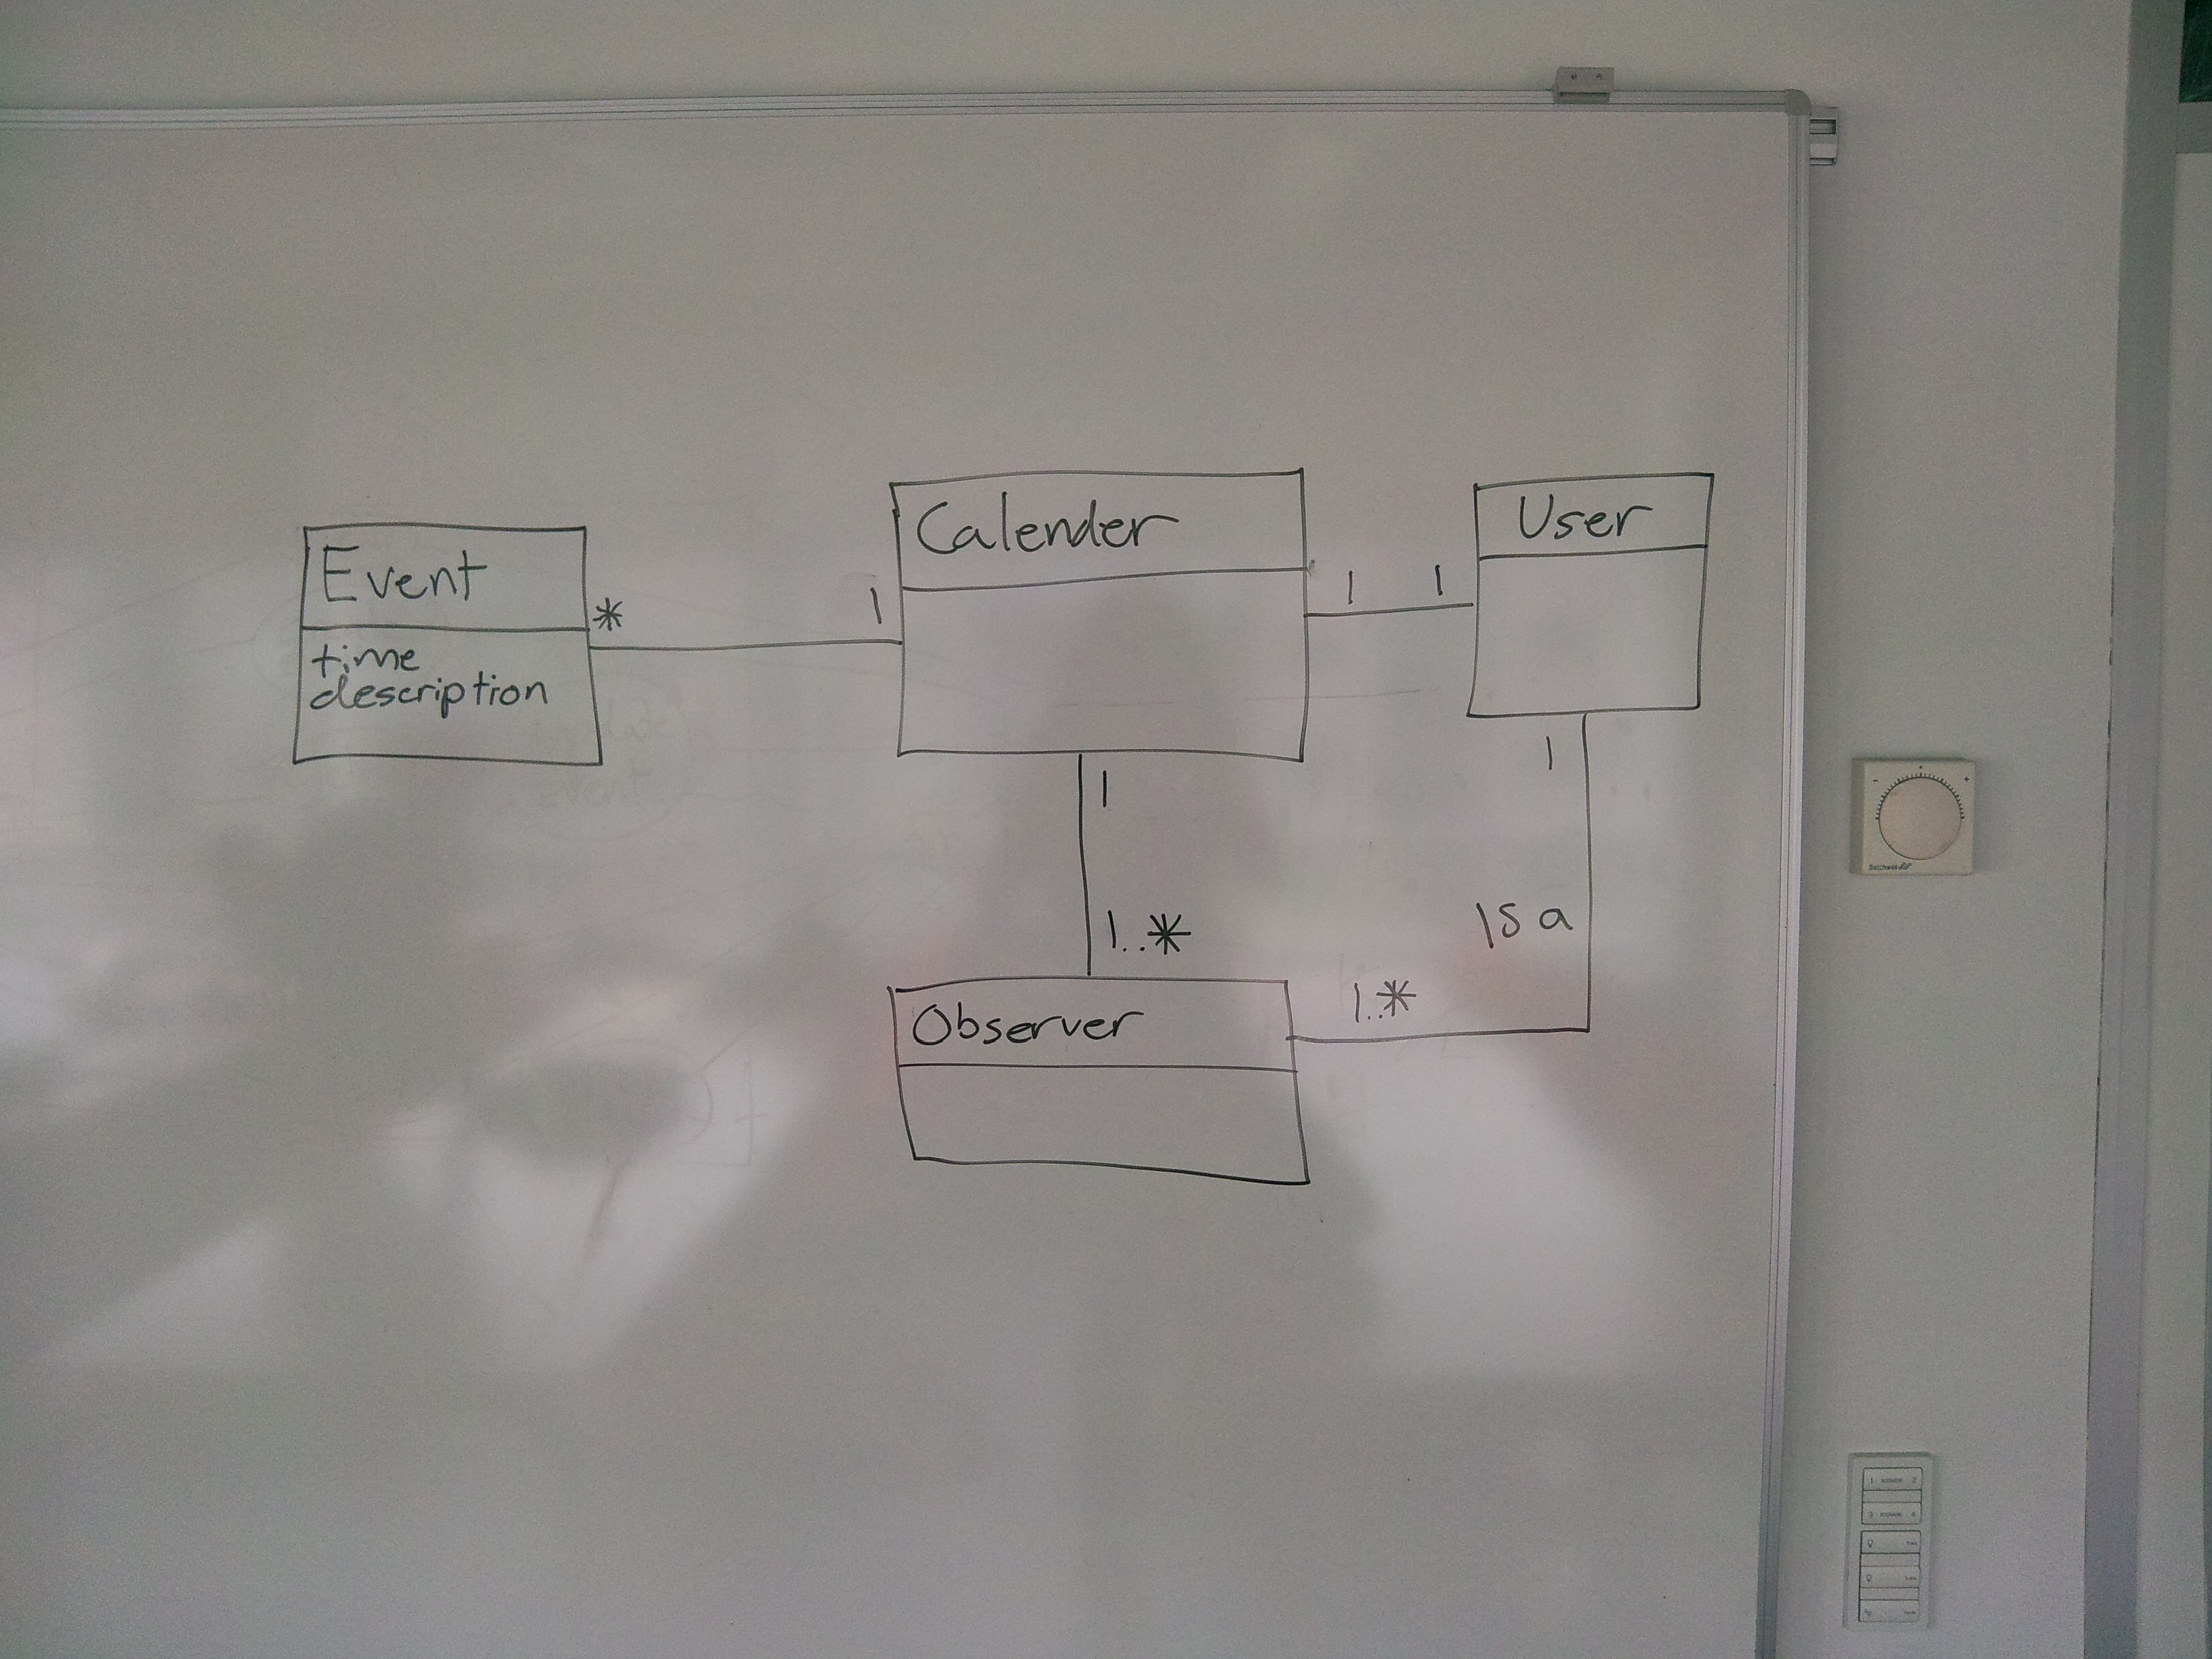
\includegraphics[width=0.7\textwidth]{./domainmodel}\\[1cm] 
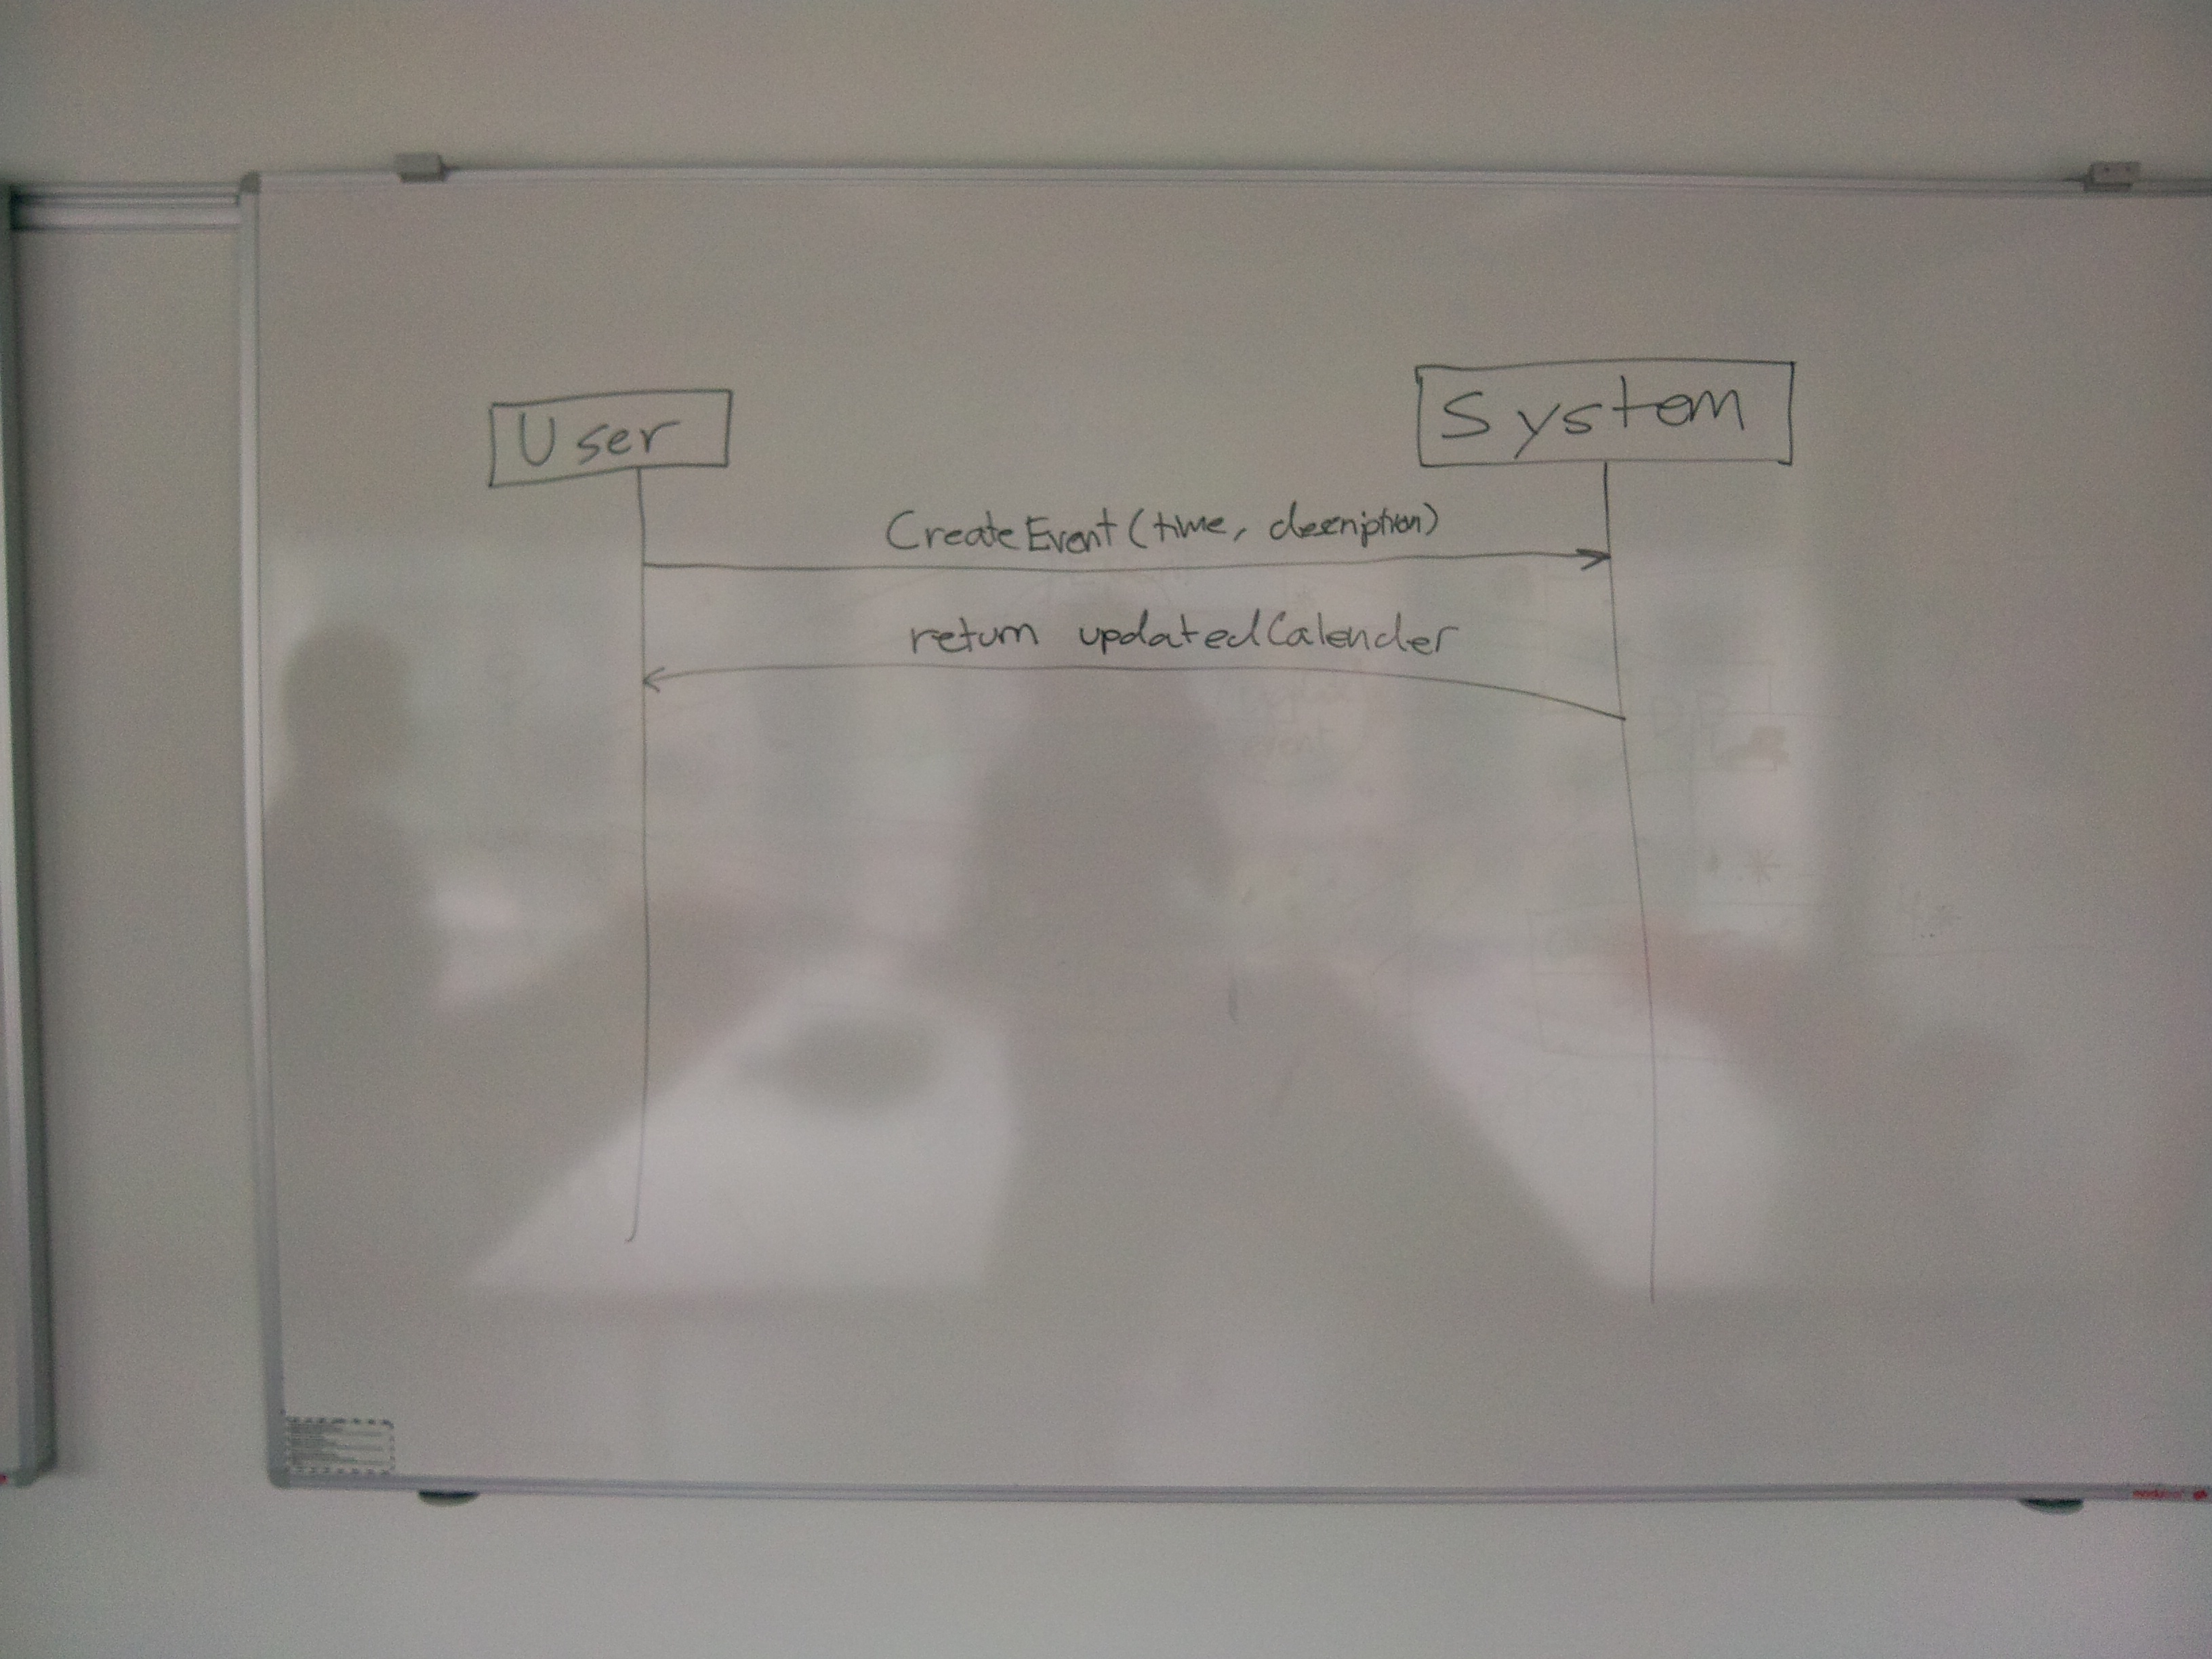
\includegraphics[width=0.7\textwidth]{./ssd}\\[1cm] 
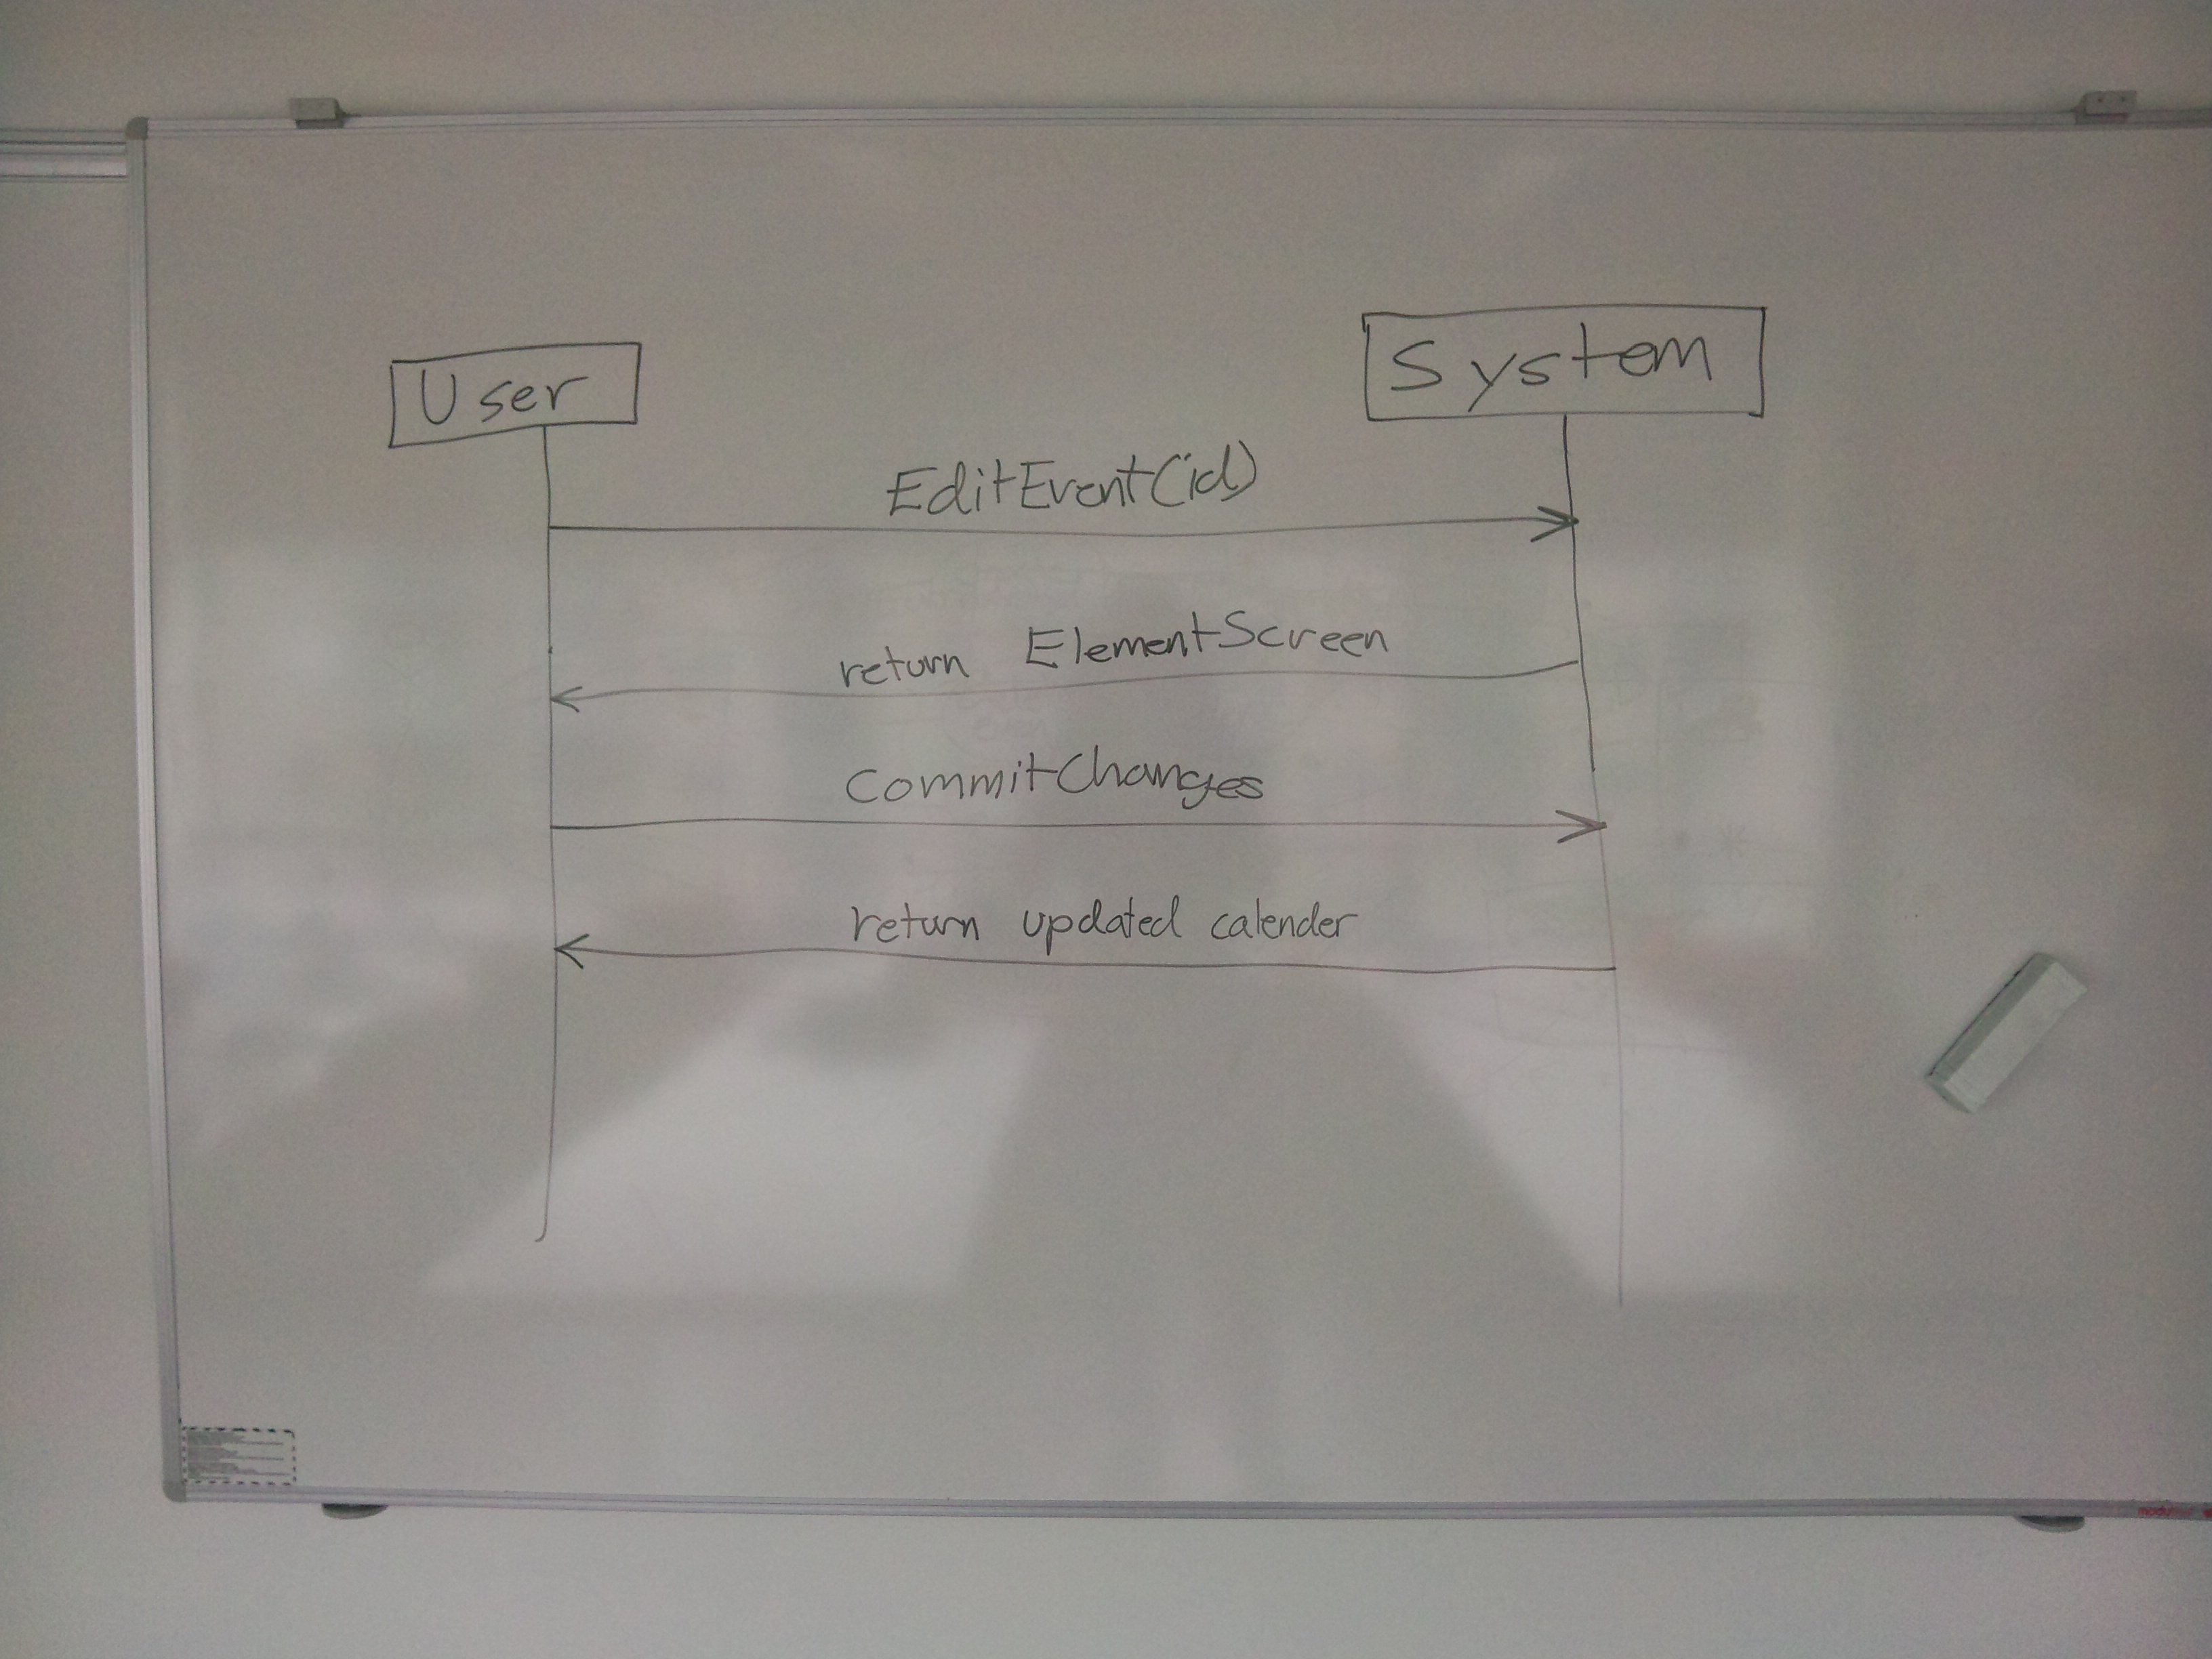
\includegraphics[width=0.7\textwidth]{./ssd2}\\[1cm] 
	
	
	
	
\end{document}